\documentclass[a4paper, 14pt, dvipdfmx]{extarticle}

\usepackage{animate}
\usepackage{amsmath, amssymb, amsthm, mathrsfs, amsfonts, dsfont}
\usepackage{ascmac}
\usepackage{bbm}
\usepackage{bm}
\usepackage{breakcites}
\usepackage{calc}
\usepackage[style=base]{caption}
\usepackage{enumerate}
\usepackage[T1]{fontenc}
\usepackage{ifthen}
\usepackage{mathtools}
\usepackage{makecell}
\usepackage{mlmodern}
\usepackage{newtxtext}
\usepackage{optidef}
\usepackage[deluxe]{otf}
\usepackage{physics}
\usepackage{pifont}
\usepackage{setspace}
\usepackage{stfloats}
\usepackage{subcaption}
\usepackage{svg}
\usepackage{tikz}
\usepackage{xparse}
\usepackage[all]{xy}

\usepackage{float}
\usepackage{color}
\usepackage{graphicx}
\usepackage[margin=20truemm]{geometry}
\usepackage[colorlinks=true, allcolors=blue]{hyperref}


% === Commands ===

\definecolor{cA}{HTML}{0072BD}
\definecolor{cB}{HTML}{EDB120}
\definecolor{cC}{HTML}{77AC30}
\definecolor{cD}{HTML}{D95319}
\definecolor{cE}{HTML}{7E2F8E}
\newcommand{\cAText}[1]{\textcolor{cA}{#1}}
\newcommand{\cBText}[1]{\textcolor{cB}{#1}}
\newcommand{\cCText}[1]{\textcolor{cC}{#1}}
\newcommand{\cDText}[1]{\textcolor{cD}{#1}}
\newcommand{\cEText}[1]{\textcolor{cE}{#1}}
\newcommand{\red}[1]{\textcolor{red}{#1}}
\newcommand{\blue}[1]{\textcolor{blue}{#1}}
\newcommand{\green}[1]{\textcolor{green}{#1}}
\newcommand{\gray}[1]{\textcolor{gray}{#1}}
\newcommand{\black}[1]{\textcolor{black}{#1}}

\newcommand{\st}{\text{ s.t. }}
\newcommand{\Img}[1]{\mathrm{Im}\qty(#1)}
\newcommand{\Ker}[1]{\mathrm{Ker}\qty(#1)}
\newcommand{\Supp}[1]{\mathrm{supp}\qty(#1)}
\newcommand{\Rank}[1]{\mathrm{rank}\qty(#1)}
\newcommand{\floor}[1]{\left\lfloor #1 \right\rfloor}
\newcommand{\ceil}[1]{\left\lceil #1 \right\rceil}
% C++ (https://tex.stackexchange.com/questions/4302/prettiest-way-to-typeset-c-cplusplus)
\newcommand{\Cpp}{C\nolinebreak[4]\hspace{-.05em}\raisebox{.4ex}{\relsize{-3}{\textbf{++}}}}
% https://tex.stackexchange.com/questions/28836/typesetting-the-define-equals-symbol
\newcommand{\defeq}{\coloneqq}
\newcommand{\eqdef}{\eqqcolon}
% https://tex.stackexchange.com/questions/5502/how-to-get-a-mid-binary-relation-that-grows
\newcommand{\relmiddle}[1]{\mathrel{}\middle#1\mathrel{}}
\newcommand{\cmark}{\cCText{\ding{51}}} % check mark
\newcommand{\xmark}{\cDText{\ding{55}}} % cross mark

\DeclareMathOperator{\Proj}{Proj}
\DeclareMathOperator{\Exp}{Exp}
\DeclareMathOperator{\Hess}{Hess}
\DeclareMathOperator{\Retr}{Retr}
\DeclareMathOperator{\Span}{span}
\DeclareMathOperator{\myGrad}{grad}
\renewcommand{\grad}{\myGrad}

% https://tex.stackexchange.com/questions/564216/newcommand-for-each-letter
\ExplSyntaxOn
\NewDocumentCommand{\definealphabet}{mmmm}{
\int_step_inline:nnn{`#3}{`#4}{
\cs_new_protected:cpx{#1 \char_generate:nn{##1}{11}}{
\exp_not:N #2{\char_generate:nn{##1}{11}}}}}
\ExplSyntaxOff

\definealphabet{bb}{\mathbb}{A}{Z}
\definealphabet{rm}{\mathrm}{A}{Z}
\definealphabet{cal}{\mathcal}{A}{Z}
% \definealphabet{scr}{\mathscr}{A}{Z}
\definealphabet{frak}{\mathfrak}{a}{z}
\definealphabet{frak}{\mathfrak}{A}{Z}

% === Settings ===

% https://qiita.com/rityo_masu/items/efd44bc8f9229e014237
\allowdisplaybreaks[4]

\usetikzlibrary{
  3d,
  fit,
  calc,
  math,
  matrix,
  patterns,
  backgrounds,
  arrows.meta,
  decorations.pathmorphing,
}

\newcommand{\IMG}[2]{
    \begin{figure}[H]
        \centering
        \includegraphics[width={#2}\columnwidth]{#1}
    \end{figure}
}

\begin{document}

\title{Supplemental Material For 10/02\\Book Reading Seminar}
\author{Hiroki Hamaguchi}
\date{\today}
\maketitle

\begin{abstract}
    \begin{center}
        This is the supplemental material for the book reading seminar.

        Please refer to the textbook and the whiteboard for the main content.

        If necessary, please also refer to the \href{https://github.com/hari64boli64/BookReadingSeminarMaterials}{repository}.

        The textbook is available at \href{https://link-springer-com.utokyo.idm.oclc.org/book/10.1007/978-3-319-91578-4}{here}.

        I recommend you to download the book from

        ``Nonsmooth Convex Optimization Pages 139-240 Download chapter PDF ''.

        \begin{figure}[htbp]
            \centering
            
\includegraphics[width=0.2\columnwidth]{../BookQR.png}
        \end{figure}

    \end{center}
\end{abstract}

\section*{p.61 Def 2.1.1 / p.139-142 Preliminary}

\begin{figure}[htbp]
    \centering
    \begin{tikzpicture}[scale=0.75]
        \begin{scope}[xshift=-5.5cm]
            \draw[thick] (-5,0) -- (5,0);
            \draw[thick, dashed] (-2.5,4) -- (-2.5,2.5);
            \draw[thick, dashed] ( 2.5,4) --   (2.5,2.5);
            \draw[thick] (-2.5,2.5) to[out=-60,in=240] (2.5,2.5);

            \draw[thick] (5,4) node {$+\infty$}; % Minus infinity symbol
            \draw[thick] (-2.5,3) node {$\approx$}; % Approximately equal symbol
            \draw[thick] (+2.5,3) node {$\approx$};  % Approximately equal symbol
            \draw[thick] (-2.5,4) -- (-4,4);
            \draw[thick] (+2.5,4) -- (+4,4);

            \filldraw[draw=black,fill=black] (-2.5,2.5) circle (3pt);
            \filldraw[draw=black,fill=white] (+2.5,2.5) circle (3pt);
            \filldraw[draw=black,fill=white] (-2.5,4) circle (3pt);
            \filldraw[draw=black,fill=black] (+2.5,4) circle (3pt);
        \end{scope}
        \begin{scope}[xshift=+5.5cm]
            \draw[thick] (-5,0) -- (5,0);
            \draw[thick, dashed] (-2.5,-2) -- (-2.5,2.5);
            \draw[thick, dashed] ( 2.5,-2) --   (2.5,2.5);
            \draw[thick] (-2.5,2.5) to[out=-60,in=240] (2.5,2.5);

            \draw[thick] (-5,-2) node {$-\infty$}; % Minus infinity symbol
            \draw[thick] (-2.5,-1) node {$\approx$}; % Approximately equal symbol
            \draw[thick] (+2.5,-1) node {$\approx$};  % Approximately equal symbol
            \draw[thick] (-2.5,-2) -- (-4,-2);
            \draw[thick] (+2.5,-2) -- (+4,-2);

            \filldraw[draw=black,fill=black] (-2.5,2.5) circle (3pt);
            \filldraw[draw=black,fill=white] (+2.5,2.5) circle (3pt);
            \filldraw[draw=black,fill=white] (-2.5,-2) circle (3pt);
            \filldraw[draw=black,fill=black] (+2.5,-2) circle (3pt);
        \end{scope}
    \end{tikzpicture}
\end{figure}

\subsection*{p.141 Lem 3.1.1 Jensen's Inequality, Col 3.1.1, 3.1.2, Thm 3.1.1}

\begin{figure}[H]
    \centering
    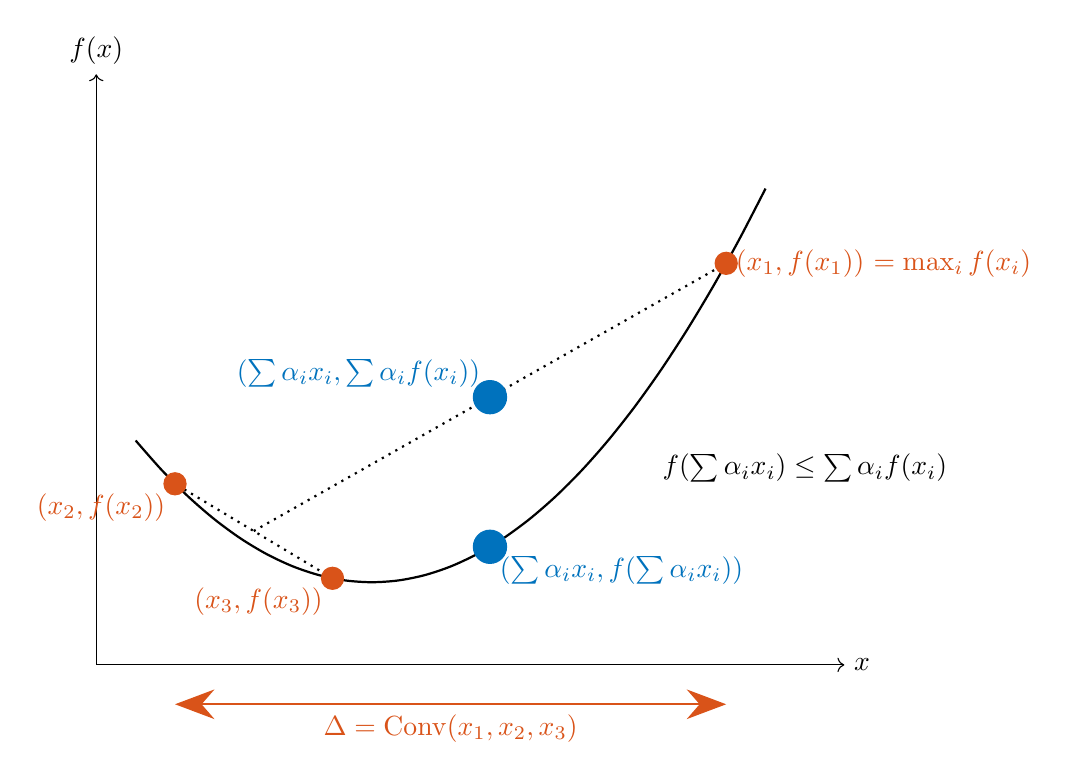
\begin{tikzpicture}
        \def\xone{3} \def\xtwo{-4} \def\xthree{-2} \def\weightedx{0}
        \def\f(#1){(0.2*#1*#1 + 0.6*#1)} % Define the function f(x)

        \draw[->] (-5,-1.5) -- (4.5,-1.5) node[right] {$x$};
        \draw[->] (-5,-1.5) -- (-5,6) node[above] {$f(x)$};
        \draw[domain=-4.5:3.5, smooth, thick] plot ({\x}, {\f(\x)});
        \draw[dotted, thick] (\xthree, {\f(\xthree)}) -- (\xtwo, {\f(\xtwo)});
        \draw[dotted, thick] ({0.5*\xthree+0.5*\xtwo}, {0.5*\f(\xthree) + 0.5*\f(\xtwo)}) -- (\xone, {\f(\xone)});

        \filldraw[cA] (\weightedx, {\f(\weightedx)}) circle (6pt) node[below right] {$(\sum \alpha_i x_i, f(\sum \alpha_i x_i))$};
        \filldraw[cA] (\weightedx, {0.5*\f(\xone) + 0.25*\f(\xtwo) + 0.25*\f(\xthree)}) circle (6pt) node[above left] {$(\sum \alpha_i x_i, \sum \alpha_i f(x_i))$};

        \node at (4,1) {$f(\sum \alpha_i x_i) \leq \sum \alpha_i f(x_i)$};

        \foreach \x/\name/\pos/\desc in {\xone/x_1/right/$= \max_{i} f(x_i)$, \xtwo/x_2/below left/, \xthree/x_3/below left/} {
                \filldraw[cD] (\x, {\f(\x)}) circle (4pt) node[\pos] {$(\name, f(\name))$ \desc};
            }

        \draw[cD, thick, {Stealth[length=5mm]}-{Stealth[length=5mm]}] (\xtwo, -2) -- (\xone, -2) node[midway, below] {$\Delta = \mathrm{Conv}(x_1, x_2, x_3)$};
    \end{tikzpicture}
\end{figure}

$\because$ induction on $n$.

\section*{p.142 Thm 3.1.2}

\begin{equation*}
    \text{$f$ is convex} \iff
    \text{$\mathrm{epi}(f)$ is a convex set}.
\end{equation*}

\begin{figure}[H]
    \centering
    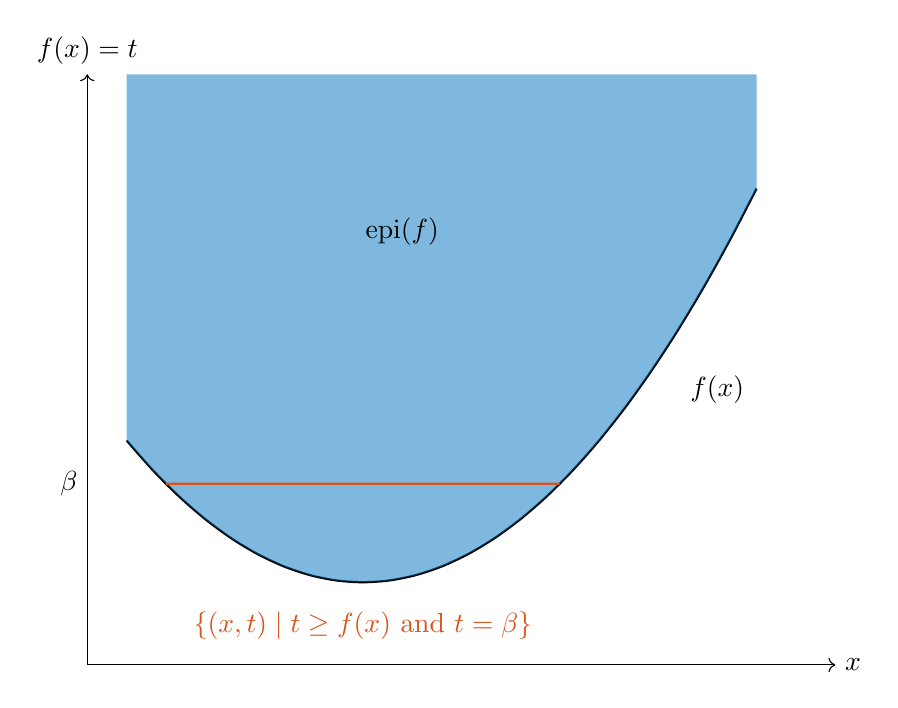
\begin{tikzpicture}
        \def\f(#1){(0.2*#1*#1 + 0.6*#1)} % Define the function f(x)

        \draw[->] (-5,-1.5) -- (4.5,-1.5) node[right] {$x$};
        \draw[->] (-5,-1.5) -- (-5,6) node[above] {$f(x)=t$};
        \draw[domain=-4.5:3.5, smooth, thick] plot ({\x}, {\f(\x)});

        % Fill the epigraph area
        \fill[cA, opacity=0.5] (-4.5, 6) -- plot[domain=-4.5:3.5] ({\x}, {\f(\x)}) -- (3.5, 6) -- cycle;

        \node at (-1,4) {$\mathrm{epi}(f)$};
        \node at (3,2) {$f(x)$};

        \draw[cD, thick] (-4, {\f(-4)}) -- (1, {\f(1)}) node[midway, below=1.5cm] {$\{ (x,t) \mid t \geq f(x) \text{ and } t=\beta \}$};
        \node[left] at (-5, {\f(-4)}) {$\beta$};
    \end{tikzpicture}
\end{figure}

\section*{p.143 Thm 3.1.3}\label{thm:3.1.3}

\begin{equation*}
    \text{All level sets } \mathscr{L}_f(\beta) = \{ x \in \mathrm{dom} f | f(x) \leq \beta \} \text{ are either convex or empty}.
\end{equation*}

\begin{figure}[H]
    \centering
    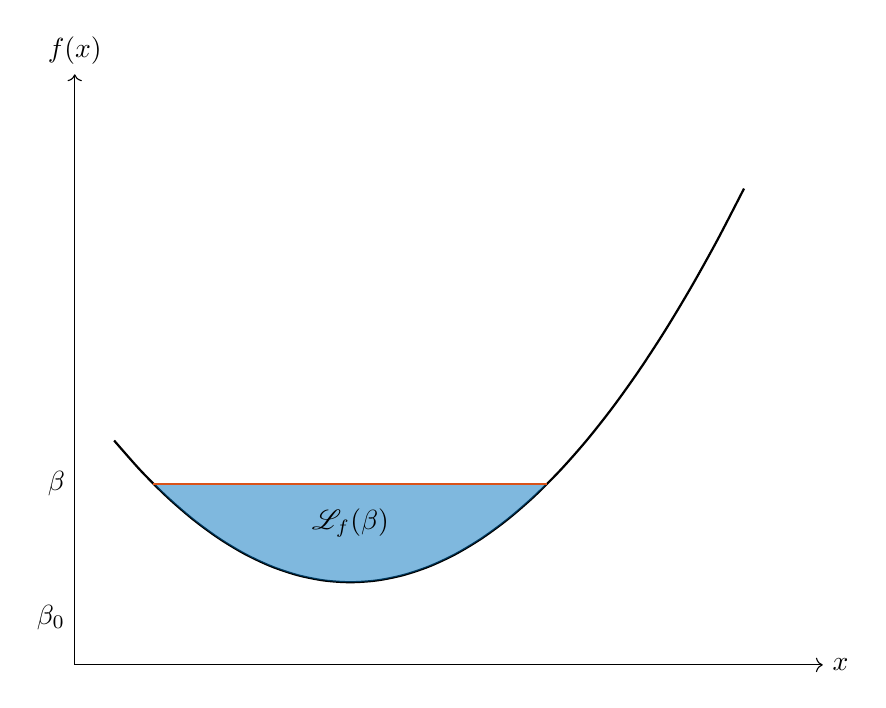
\begin{tikzpicture}
        \def\f(#1){(0.2*#1*#1 + 0.6*#1)} % Define the function f(x)
        \def\Beta{\f(-4)} % Define the value of 

        \draw[->] (-5,-1.5) -- (4.5,-1.5) node[right] {$x$};
        \draw[->] (-5,-1.5) -- (-5,6) node[above] {$f(x)$};
        \draw[domain=-4.5:3.5, smooth, thick] plot ({\x}, {\f(\x)});

        % Fill the level set area
        \fill[cA, opacity=0.5] (-4, {\Beta}) -- plot[domain=-4:1] ({\x}, {\f(\x)}) -- (1, {\Beta}) -- cycle;

        % Draw the level set line at f(x) = \Beta
        \draw[cD, thick] (-4, {\Beta}) -- (1, {\Beta});
        \node[left] at (-5, {\Beta}) {$\beta$};
        \node[left] at (-5, {\Beta-1.7}) {$\beta_0$};

        % Label for the level set
        \node at (-1.5, {\Beta-0.5}) {$\mathscr{L}_f(\beta)$};
    \end{tikzpicture}
\end{figure}

\section*{p.143 Def 3.1.2}\label{def:3.1.2}

1d version of Example 3.1.1(6):
\begin{equation*}
    f(x) = \begin{dcases}
        0      & (-1 \leq x \leq 1)     \\
        1      & (x=-1 \text{ or } x=1) \\
        \infty & (\text{otherwise})     \\
    \end{dcases}.
\end{equation*}

\begin{figure}[H]
    \centering
    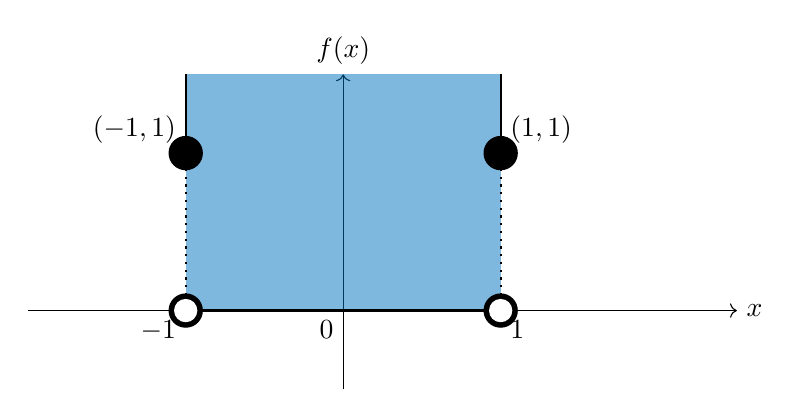
\begin{tikzpicture}
        \begin{scope}[xscale=2.0,yscale=2.0]
            \draw[->] (-2,0) -- (2.5,0) node[right] {$x$};
            \draw[->] (0,-0.5) -- (0,1.5) node[above] {$f(x)$};

            \fill[cA, opacity=0.5] (-1,0) -- (-1,1.5) -- (1,1.5) -- (1,0) -- cycle;

            \draw[thick] (-1,0) -- (1,0);
            \draw[thick,dotted] (-1, 0) -- (-1, 1);
            \draw[thick] (-1, 1) -- (-1, 1.5);
            \draw[thick,dotted] (1, 0) -- (1, 1);
            \draw[thick] (1, 1) -- (1, 1.5);

            \filldraw (-1,0) circle (3pt);
            \filldraw (1,0) circle (3pt);
            \filldraw[white] (-1,0) circle (2pt);
            \filldraw[white] (1,0) circle (2pt);

            \filldraw (-1,1) circle (3pt) node[above left] {$( -1, 1 )$};
            \filldraw (1,1) circle (3pt) node[above right] {$( 1, 1 )$};

            \node[below left] at (-1,0) {$-1$};
            \node[below right] at (1,0) {$1$};
            \node[below left] at (0,0) {$0$};
        \end{scope}
    \end{tikzpicture}
\end{figure}

To exclude such a \footnote{病的な}{pathological} case,
we define the constrained epigraph set $\mathrm{epi}_Q(f)$ and closed convex function.

\begin{figure}[H]
    \centering
    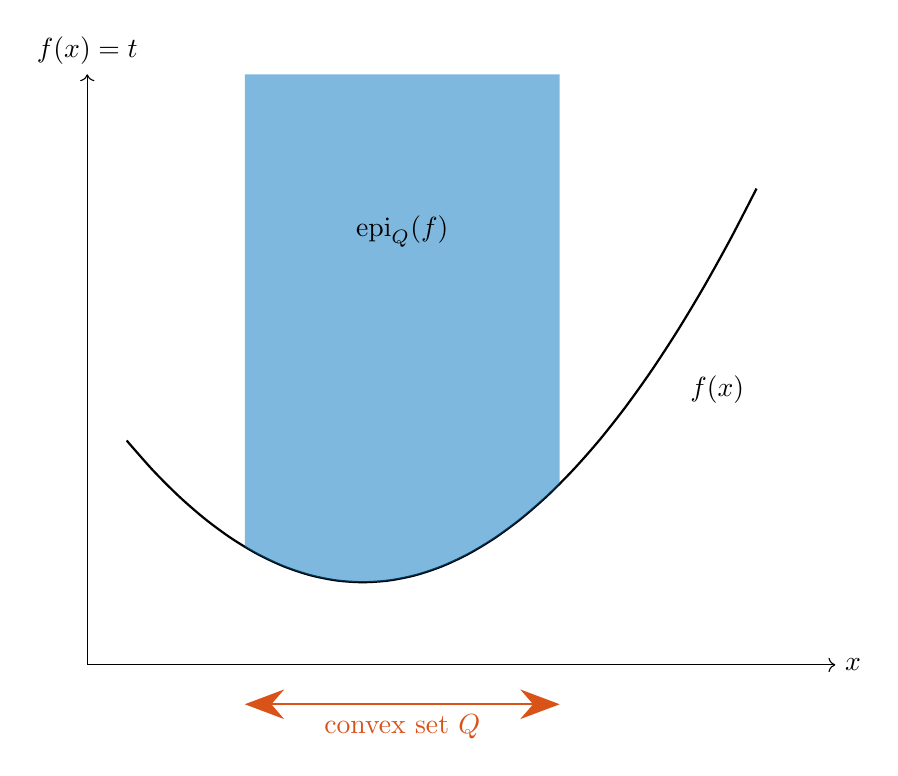
\begin{tikzpicture}
        \def\f(#1){(0.2*#1*#1 + 0.6*#1)} % Define the function f(x)

        \draw[->] (-5,-1.5) -- (4.5,-1.5) node[right] {$x$};
        \draw[->] (-5,-1.5) -- (-5,6) node[above] {$f(x)=t$};
        \draw[domain=-4.5:3.5, smooth, thick] plot ({\x}, {\f(\x)});

        % Fill the epigraph area
        \fill[cA, opacity=0.5] (-3, 6) -- plot[domain=-3:1] ({\x}, {\f(\x)}) -- (1, 6) -- cycle;

        \node at (-1,4) {$\mathrm{epi}_Q(f)$};
        \node at (3,2) {$f(x)$};

        \draw[cD, thick, {Stealth[length=5mm]}-{Stealth[length=5mm]}] (-3, -2) -- (1, -2) node[midway, below] {convex set $Q$};
    \end{tikzpicture}
\end{figure}

\section*{p.144 Lem 3.1.2}

subset of closed convex set.

\begin{itembox}[l]{Thm 2.2.8}
    Let $Q_1 \subseteq \bbR^n$ and $Q_2 \subseteq \bbR^n$ be closed convex sets, and $\mathscr{A}(\cdot)$ be a linear operator:
    \begin{equation*}
        \mathscr{A}(x) = Ax+b: \bbR^n \to \bbR^m.
    \end{equation*}
    \begin{enumerate}
        \item The intersection of two sets($m=n$), $Q_1 \cap Q_2 = \{ x \in \bbR^n | x \in Q_1, x \in Q_2 \}$, is convex and closed.
        \item $\dots$
    \end{enumerate}
\end{itembox}

\section*{p.144 Thm 3.1.4}

\subsection*{1}\label{lem:3.1.4.1}

Sometimes, the convex function is treated as a continuous function (\href{https://mathlandscape.com/convex-func}{example}), but in this book, that is not the case.

\IMG{convexIsContinuous.png}{0.8}

This is because the definition is different.

The lower semi-continuous by wikipedia:
\IMG{lowerSemiContinuous.png}{0.5}

We use the following facts to prove the theorem.
See \href{https://mathlandscape.com/limsup-liminf/}{here} for proof.
\begin{itemize}
    \item If the terms in the sequence are real numbers, the limit superior and limit inferior always exist.
          (i.e. $\liminf_{k\to\infty} f(x_k) \in \bbR \cup \{\pm\infty\}$)
    \item If $\liminf_{k\to\infty} f(x_k) \to \beta$ where $\beta \in \bbR$, then there exists a subsequence $\{ x_{k_j} \}$ such that $\lim_{j\to\infty} f(x_{k_j}) = \beta$.
    \item The assertion above implies that if there are no convergent subsequences, then $\liminf_{k\to\infty} f(x_k) \in \{\pm\infty\}$.
\end{itemize}

\IMG{img0.png}{0.8}
\IMG{img1.png}{0.8}
\IMG{img2.png}{0.8}
\IMG{img3.png}{0.8}
\IMG{img4.png}{0.8}
\IMG{img5.png}{0.8}

\IMG{psi.png}{0.8}

\IMG{why_interval_1.pdf}{0.8}
\IMG{why_interval_2.png}{0.8}

\subsection*{2}

whiteboard.

\subsection*{3}

Please see \href{thm:3.1.3}{thm 3.1.3}.

\subsection*{4}

whiteboard.

\subsection*{5}

whiteboard.


\section*{p.145 Example 3.1.1}

\subsection*{4}

\begin{figure}[H]
    \centering
    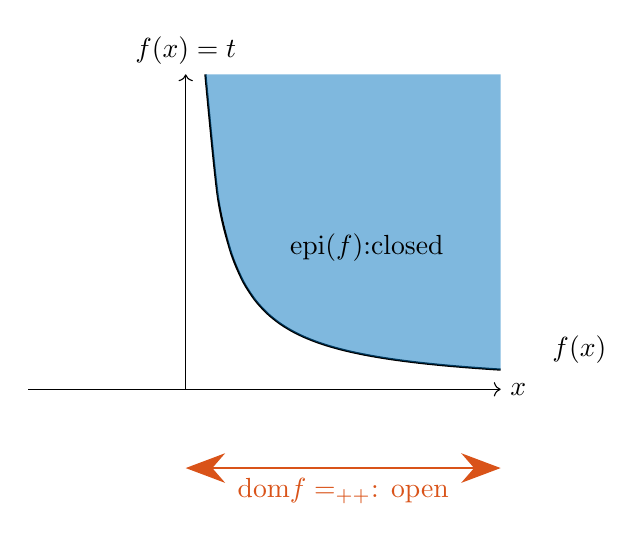
\begin{tikzpicture}
        \def\f(#1){(1/#1)} % Define the function f(x)

        \draw[->] (-2,0) -- (4,0) node[right] {$x$};
        \draw[->] (0,0) -- (0,4) node[above] {$f(x)=t$};
        \draw[domain=0.25:4, smooth, thick] plot ({\x}, {\f(\x)});

        % Fill the epigraph area
        \fill[cA, opacity=0.5] (0.25, 4) -- plot[domain=0.25:4] ({\x}, {\f(\x)}) -- (4, 4) -- cycle;

        \node at (2.3,1.8) {$\mathrm{epi}(f)$:closed};
        \node at (5,0.5) {$f(x)$};

        \draw[cD, thick, {Stealth[length=5mm]}-{Stealth[length=5mm]}] (0, -1) -- (4, -1) node[midway, below] {$\mathrm{dom} f=\bbR_{++}$: open};
    \end{tikzpicture}
\end{figure}

\subsection*{5}

\begin{figure}[H]
    \centering
    \begin{tikzpicture}
        \begin{scope}[scale=2]
            % Axes
            \draw[->] (-2.5,0) -- (2.5,0) node[right] {$x_1$};
            \draw[->] (0,-2.5) -- (0,2.5) node[above] {$x_2$};

            % L1 norm unit ball (diamond)
            \draw[cA, thick] (0,1) -- (1,0) -- (0,-1) -- (-1,0) -- cycle;
            \node[cA] at (-1.5, 1.5) {$L_1$};

            % L2 norm unit ball (circle)
            \draw[cB, thick] (0,0) circle (1);
            \node[cB] at (1.5, 1.5) {$L_2$};

            % Lp norm unit ball (p=4, rounded square)
            \draw[cC, thick, domain=0:90, smooth, variable=\t] plot ({(cos(\t))^(2/4)}, {(sin(\t))^(2/4)});
            \draw[cC, thick, domain=0:90, smooth, variable=\t] plot ({-((cos(\t))^(2/4))}, {(sin(\t))^(2/4)});
            \draw[cC, thick, domain=0:90, smooth, variable=\t] plot ({-((cos(\t))^(2/4))}, {-((sin(\t))^(2/4))});
            \draw[cC, thick, domain=0:90, smooth, variable=\t] plot ({(cos(\t))^(2/4)}, {-((sin(\t))^(2/4))});
            \node[cC] at (1.5, -1.5) {$L_p$ ($p=4$)};

            % L-infinity norm unit ball (square)
            \draw[cD, thick] (-1,-1) -- (-1,1) -- (1,1) -- (1,-1) -- cycle;
            \node[cD] at (-1.5, -1.5) {$L_\infty$};
        \end{scope}
    \end{tikzpicture}
\end{figure}

\subsection*{6}

Please see \href{def:3.1.2}{def 3.1.2}.

\section*{p.147 Thm 3.1.5}

\subsection*{3}

\begin{figure}[H]
    \centering
    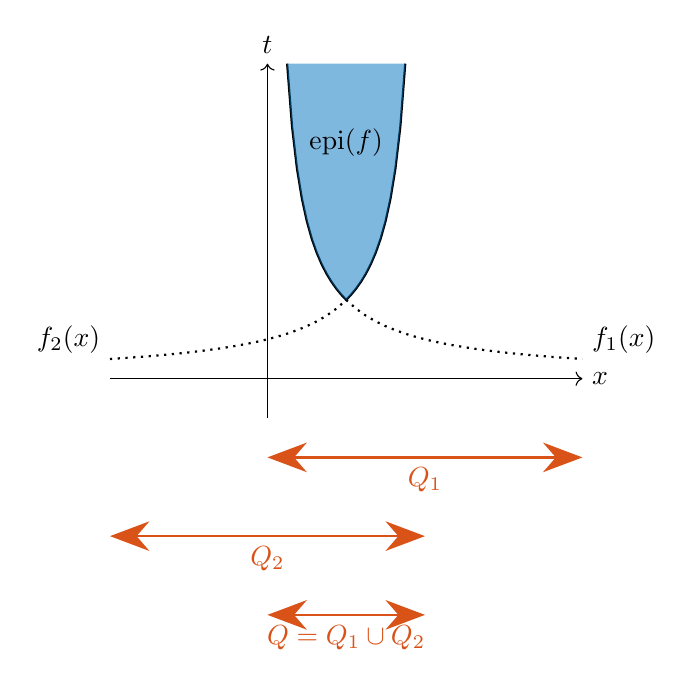
\begin{tikzpicture}
        \def\fA(#1){1/(#1)}      % f_1(x) = 1/x
        \def\fB(#1){1/(2-#1)}    % f_2(x) = 1/(2-x)
        \def\f(#1){max(1/(#1), 1/(2-#1))} % f(x) = max(f_1(x), f_2(x))

        % Axes
        \draw[->] (-2,0) -- (4,0) node[right] {$x$};
        \draw[->] (0,-0.5) -- (0,4) node[above] {$t$};

        % Plot f_1(x) and f_2(x) as dotted lines
        \draw[domain=1:4, dotted, thick] plot (\x, {\fA(\x)});
        \node[right] at (4,0.5) {$f_1(x)$};
        \draw[domain=-2:1, dotted, thick] plot (\x, {\fB(\x)});
        \node[left] at (-2,0.5) {$f_2(x)$};

        % Plot max(f_1(x), f_2(x)) as a solid line
        \draw[domain=0.25:1.75, thick] plot (\x, {\f(\x)});

        % Fill the epigraph area of f(x)
        \fill[cA, opacity=0.5] (0.25, 4) -- plot[domain=0.25:1] ({\x}, {\fA(\x)}) -- plot[domain=1:1.75] ({\x}, {\fB(\x)}) -- (1.75, 4) -- cycle;

        % Label for the epigraph of f(x)
        \node at (1,3) {$\mathrm{epi}(f)$};

        % Draw arrows for intervals
        \draw[cD, thick, {Stealth[length=5mm]}-{Stealth[length=5mm]}] (0,-1) -- (4,-1) node[midway, below] {$Q_1$};
        \draw[cD, thick, {Stealth[length=5mm]}-{Stealth[length=5mm]}] (-2,-2) -- (2,-2) node[midway, below] {$Q_2$};
        \draw[cD, thick, {Stealth[length=5mm]}-{Stealth[length=5mm]}] (0,-3) -- (2,-3) node[midway, below] {$Q = Q_1 \cup Q_2$};

    \end{tikzpicture}
\end{figure}

\section*{p.148 Thm 3.1.6}

affine-invariant. whiteboard.

\section*{p.149 Thm 3.1.7}

inf of $\phi(x,y)$. whiteboard.

\section*{p.149 Thm 3.1.8}

\begin{figure}[H]
    \centering
    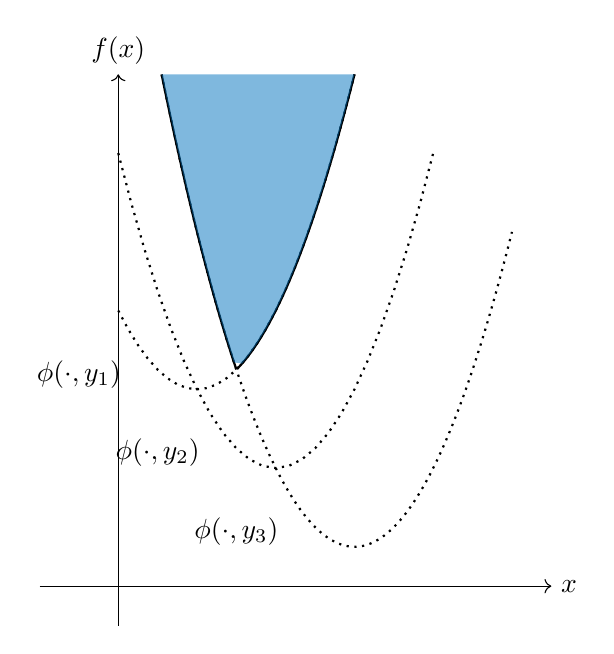
\begin{tikzpicture}
        % Define functions f_1, f_2, and f_3
        \def\fA(#1){2.5 + (#1-1)^2}      % f_1(x) = 2.5 + (x-1)^2
        \def\fB(#1){1.5 + (#1-2)^2}      % f_2(x) = 1.5 + (x-2)^2
        \def\fC(#1){0.5 + (#1-3)^2}      % f_3(x) = 0.5 + (x-3)^2
        \def\f(#1){max(\fA(#1),\fB(#1),\fC(#1))} % f(x) = max(f_1(x), f_2(x), f_3(x))

        % Axes
        \draw[->] (-1,0) -- (5.5,0) node[right] {$x$};
        \draw[->] (0,-0.5) -- (0,6.5) node[above] {$f(x)$};

        % Plot f_1(x), f_2(x), f_3(x)
        \draw[domain=0:3, dotted, thick] plot (\x, {\fA(\x)}) node[below] at (-0.5,3) {$\phi(\cdot,y_1)$};
        \draw[domain=0:4, dotted, thick] plot (\x, {\fB(\x)}) node[below] at (0.5,2) {$\phi(\cdot,y_2)$};
        \draw[domain=0.551:5, samples=100, dotted, thick] plot (\x, {\fC(\x)}) node[below] at (1.5,1) {$\phi(\cdot,y_3)$};

        % Plot max(f_1(x), f_2(x), f_3(x)) as a solid line
        \draw[domain=0.551:3, samples=100, thick] plot (\x, {\f(\x)});

        % Fill the epigraph of max(f_1, f_2, f_3)
        \fill[cA, opacity=0.5] (0.551, 6.5) -- plot[domain=0.551:3] (\x, {\f(\x)}) -- (3, 6.5) -- cycle;
    \end{tikzpicture}
\end{figure}

\section*{p.150 Thm 3.1.9}

composition of convex functions. whiteboard.

\section*{p.150 Example 3.1.2}

\subsection*{1}

My favorite explanation of Fenchel conjugate: \href{https://qiita.com/wosugi/items/8d5a407a0a0434aaabeb}{link}

\animategraphics[loop,controls,width=\columnwidth]{10}{conj1/conj1-}{0}{96}

\animategraphics[loop,controls,width=\columnwidth]{10}{conj2/conj2-}{0}{64}

\subsection*{3}

\begin{figure}[H]
    \centering
    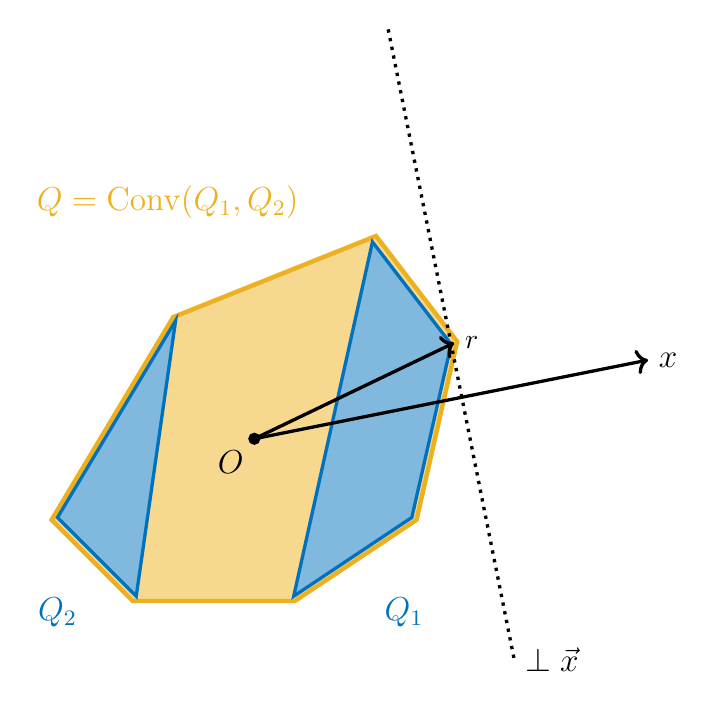
\begin{tikzpicture}
        \coordinate (A) at (-2.5,-1);
        \coordinate (B) at (-1,1.5);
        \coordinate (C) at (1.5,2.5);
        \coordinate (D) at (2.5,1.2);
        \coordinate (E) at (2.0,-1);
        \coordinate (F) at (0.5,-2);
        \coordinate (G) at (-1.5,-2);

        \draw[cB, fill=cB!50!white, ultra thick] ($1.03*(A)$) -- ($1.03*(B)$) -- ($1.03*(C)$) -- ($1.03*(D)$) -- ($1.03*(E)$) -- ($1.03*(F)$) -- ($1.03*(G)$) -- cycle;
        \draw[cA, fill=cA!50!white, very thick] (C) -- (D) -- (E) -- (F) -- cycle;
        \draw[cA, fill=cA!50!white, very thick] (A) -- (B) -- (G) -- cycle;

        \filldraw (0,0) circle (2pt);

        \node[cA] at (-2.5,-2.2) {\large $Q_2$};
        \node[cA] at (+1.9,-2.2) {\large $Q_1$};
        \node[cB] at (-1.1,+3) {\large $Q=\mathrm{Conv}(Q_1, Q_2)$};
        \node at (-0.3,-0.3) {\large $O$};

        \draw[very thick, ->] (0,0) -- ($1.015*(D)$) node[anchor=west] {$r$};

        \draw[very thick, ->] (0,0) -- (5.0,1.0) node[anchor=west] {\large $x$};
        \draw[very thick, dotted] (2.5-0.8,1.2+4) -- (2.5+0.8,1.2-4) node[anchor=west] {\large $\bot \; \vec{x}$};
    \end{tikzpicture}
\end{figure}

\subsection*{4}

Minkowski function.

For example, let us consider the case the convex function Q is $Q = \{ (x,y) \in \bbR^2 | (x-0.5)^2 + 2y^2 \leq 1 \}$.
The Minkowski function is defined as:
\begin{align*}
    f(x,y) & = \min_{\tau \geq 0} \{ \tau : (x,y) \in \tau Q \}                          \\
           & = \min_{\tau \geq 0} \{ \tau : (1/\tau x - 0.5)^2 + 2(1/\tau y)^2 \leq 1 \} \\
           & = \max_{t \geq 0} \{ t : (tx-0.5)^2 + 2(ty)^2 \leq 1 \}                     \\
           & = \max_{t \geq 0} \{ t : t^2(x^2+2y^2) - tx - 0.75 \leq 0 \}                \\
           & = \frac{\max(x \pm \sqrt{4x^2+6y^2})}{2(x^2+2y^2)}.
\end{align*}

\IMG{Minkowski.pdf}{0.8}

This is actually a convex function.

\section*{p.153 Lem 3.1.4}\label{lem:3.1.4}

Please compare with \href{lem:3.1.4.1}{lem 3.1.4.1}.

\end{document}
